\documentclass[]{article}
\usepackage{lmodern}
\usepackage{amssymb,amsmath}
\usepackage{ifxetex,ifluatex}
\usepackage{fixltx2e} % provides \textsubscript
\ifnum 0\ifxetex 1\fi\ifluatex 1\fi=0 % if pdftex
  \usepackage[T1]{fontenc}
  \usepackage[utf8]{inputenc}
\else % if luatex or xelatex
  \ifxetex
    \usepackage{mathspec}
  \else
    \usepackage{fontspec}
  \fi
  \defaultfontfeatures{Ligatures=TeX,Scale=MatchLowercase}
\fi
% use upquote if available, for straight quotes in verbatim environments
\IfFileExists{upquote.sty}{\usepackage{upquote}}{}
% use microtype if available
\IfFileExists{microtype.sty}{%
\usepackage{microtype}
\UseMicrotypeSet[protrusion]{basicmath} % disable protrusion for tt fonts
}{}
\usepackage[margin=1in]{geometry}
\usepackage{hyperref}
\hypersetup{unicode=true,
            pdftitle={EDMS 646: Homework 3},
            pdfauthor={Minoo Ahmadi},
            pdfborder={0 0 0},
            breaklinks=true}
\urlstyle{same}  % don't use monospace font for urls
\usepackage{color}
\usepackage{fancyvrb}
\newcommand{\VerbBar}{|}
\newcommand{\VERB}{\Verb[commandchars=\\\{\}]}
\DefineVerbatimEnvironment{Highlighting}{Verbatim}{commandchars=\\\{\}}
% Add ',fontsize=\small' for more characters per line
\usepackage{framed}
\definecolor{shadecolor}{RGB}{248,248,248}
\newenvironment{Shaded}{\begin{snugshade}}{\end{snugshade}}
\newcommand{\KeywordTok}[1]{\textcolor[rgb]{0.13,0.29,0.53}{\textbf{{#1}}}}
\newcommand{\DataTypeTok}[1]{\textcolor[rgb]{0.13,0.29,0.53}{{#1}}}
\newcommand{\DecValTok}[1]{\textcolor[rgb]{0.00,0.00,0.81}{{#1}}}
\newcommand{\BaseNTok}[1]{\textcolor[rgb]{0.00,0.00,0.81}{{#1}}}
\newcommand{\FloatTok}[1]{\textcolor[rgb]{0.00,0.00,0.81}{{#1}}}
\newcommand{\ConstantTok}[1]{\textcolor[rgb]{0.00,0.00,0.00}{{#1}}}
\newcommand{\CharTok}[1]{\textcolor[rgb]{0.31,0.60,0.02}{{#1}}}
\newcommand{\SpecialCharTok}[1]{\textcolor[rgb]{0.00,0.00,0.00}{{#1}}}
\newcommand{\StringTok}[1]{\textcolor[rgb]{0.31,0.60,0.02}{{#1}}}
\newcommand{\VerbatimStringTok}[1]{\textcolor[rgb]{0.31,0.60,0.02}{{#1}}}
\newcommand{\SpecialStringTok}[1]{\textcolor[rgb]{0.31,0.60,0.02}{{#1}}}
\newcommand{\ImportTok}[1]{{#1}}
\newcommand{\CommentTok}[1]{\textcolor[rgb]{0.56,0.35,0.01}{\textit{{#1}}}}
\newcommand{\DocumentationTok}[1]{\textcolor[rgb]{0.56,0.35,0.01}{\textbf{\textit{{#1}}}}}
\newcommand{\AnnotationTok}[1]{\textcolor[rgb]{0.56,0.35,0.01}{\textbf{\textit{{#1}}}}}
\newcommand{\CommentVarTok}[1]{\textcolor[rgb]{0.56,0.35,0.01}{\textbf{\textit{{#1}}}}}
\newcommand{\OtherTok}[1]{\textcolor[rgb]{0.56,0.35,0.01}{{#1}}}
\newcommand{\FunctionTok}[1]{\textcolor[rgb]{0.00,0.00,0.00}{{#1}}}
\newcommand{\VariableTok}[1]{\textcolor[rgb]{0.00,0.00,0.00}{{#1}}}
\newcommand{\ControlFlowTok}[1]{\textcolor[rgb]{0.13,0.29,0.53}{\textbf{{#1}}}}
\newcommand{\OperatorTok}[1]{\textcolor[rgb]{0.81,0.36,0.00}{\textbf{{#1}}}}
\newcommand{\BuiltInTok}[1]{{#1}}
\newcommand{\ExtensionTok}[1]{{#1}}
\newcommand{\PreprocessorTok}[1]{\textcolor[rgb]{0.56,0.35,0.01}{\textit{{#1}}}}
\newcommand{\AttributeTok}[1]{\textcolor[rgb]{0.77,0.63,0.00}{{#1}}}
\newcommand{\RegionMarkerTok}[1]{{#1}}
\newcommand{\InformationTok}[1]{\textcolor[rgb]{0.56,0.35,0.01}{\textbf{\textit{{#1}}}}}
\newcommand{\WarningTok}[1]{\textcolor[rgb]{0.56,0.35,0.01}{\textbf{\textit{{#1}}}}}
\newcommand{\AlertTok}[1]{\textcolor[rgb]{0.94,0.16,0.16}{{#1}}}
\newcommand{\ErrorTok}[1]{\textcolor[rgb]{0.64,0.00,0.00}{\textbf{{#1}}}}
\newcommand{\NormalTok}[1]{{#1}}
\usepackage{graphicx,grffile}
\makeatletter
\def\maxwidth{\ifdim\Gin@nat@width>\linewidth\linewidth\else\Gin@nat@width\fi}
\def\maxheight{\ifdim\Gin@nat@height>\textheight\textheight\else\Gin@nat@height\fi}
\makeatother
% Scale images if necessary, so that they will not overflow the page
% margins by default, and it is still possible to overwrite the defaults
% using explicit options in \includegraphics[width, height, ...]{}
\setkeys{Gin}{width=\maxwidth,height=\maxheight,keepaspectratio}
\IfFileExists{parskip.sty}{%
\usepackage{parskip}
}{% else
\setlength{\parindent}{0pt}
\setlength{\parskip}{6pt plus 2pt minus 1pt}
}
\setlength{\emergencystretch}{3em}  % prevent overfull lines
\providecommand{\tightlist}{%
  \setlength{\itemsep}{0pt}\setlength{\parskip}{0pt}}
\setcounter{secnumdepth}{0}
% Redefines (sub)paragraphs to behave more like sections
\ifx\paragraph\undefined\else
\let\oldparagraph\paragraph
\renewcommand{\paragraph}[1]{\oldparagraph{#1}\mbox{}}
\fi
\ifx\subparagraph\undefined\else
\let\oldsubparagraph\subparagraph
\renewcommand{\subparagraph}[1]{\oldsubparagraph{#1}\mbox{}}
\fi

%%% Use protect on footnotes to avoid problems with footnotes in titles
\let\rmarkdownfootnote\footnote%
\def\footnote{\protect\rmarkdownfootnote}

%%% Change title format to be more compact
\usepackage{titling}

% Create subtitle command for use in maketitle
\newcommand{\subtitle}[1]{
  \posttitle{
    \begin{center}\large#1\end{center}
    }
}

\setlength{\droptitle}{-2em}
  \title{EDMS 646: Homework 3}
  \pretitle{\vspace{\droptitle}\centering\huge}
  \posttitle{\par}
  \author{Minoo Ahmadi}
  \preauthor{\centering\large\emph}
  \postauthor{\par}
  \predate{\centering\large\emph}
  \postdate{\par}
  \date{March 9, 2017}

\usepackage{float,amsmath,siunitx,booktabs,caption}

\begin{document}
\maketitle

\begin{center}
\Large \textbf{PART 1: Multiple Regression - Initial model: Use data set HSB1}
\end{center}

\begin{enumerate}
\def\labelenumi{\arabic{enumi}.}
\item
\end{enumerate}

\[\hat{Y} = 50.3514 + 4.7188(\text{locus}) + 0.2549(\text{concept}) + 1.7113(\text{mot})\]

Controlling for self-concept and motivation, one unit increase in locus
of control will increase the science score by 4.7188 units. Controlling
for locus of control and motivation, one unit increase in self-concept
will increase the science score by 0.2549 units. Controlling for locus
of control and self-concept, one unit increase in motivation will
increase the science score by 1.7113 units.

\begin{enumerate}
\def\labelenumi{\arabic{enumi}.}
\setcounter{enumi}{1}
\item
\end{enumerate}

\(H_0\): \(\beta_{locus} = \beta_{concept} = \beta_{mot} = 0\)\\
\(H_1\): \(\beta_j \neq 0\)

The null hypothesis states that the model has no predictive capability
and all the regression coefficients equal to zero. In other words, none
of the 3 predictors (locus of control, self-concept and motivation) can
predict the outcome (science score).

The alternative hypothesis on the other hand, states that at least one
of the predictors has the capability of predicting the outcome. In other
words, at least one of the regression coefficients is significantly
different from 0.

Looking at the results from the ANOVA table, our F-value exceeds the
critical F-value and the p-value is less than .001. Therefore, at least
one of our predictors has a significant regression coefficient and we
reject the null hypothesis.

\begin{enumerate}
\def\labelenumi{\arabic{enumi}.}
\setcounter{enumi}{2}
\tightlist
\item
  As opposed to ANOVA, which is an omnibus test, regression table is
  reporting t-tests for each of the predictors.
\end{enumerate}

The null hypothesis for each of the predictors is that this specific
predictor (let it be locus of control, self-concept or motivation) has
no predictive capability for the outcome (science score) when
controlling for other predictors in the model. In other words, the true
slope is 0.

The alternative hypothesis on the other hand states that, when the other
predictors in the model are controlled for, this specific predictor
predicts the outcome and its regression coefficient is significantly
different from 0.

Based on the t-tests, it seems that locus of control is the only
predictor in our model that can significantly predict the science score
when accounting for self-concept and motivation. For locus of predictor,
the t-value exceeds the critical t-value and our p-value is less than
.001. Hence, we reject the null hypothesis.

The t-test is not significant for the concept and motivation and we
cannot conclude that they have the capability of predicting science
score.

Standard error of the regression coefficients show the variability of
the sampling distribution for the slope for each of the predictors when
accounting for the other predictors.

\begin{enumerate}
\def\labelenumi{\arabic{enumi}.}
\setcounter{enumi}{3}
\tightlist
\item
  Normality: The histogram for standarized residulas seems left-skewed.
\end{enumerate}

\begin{table}[H]
\centering
\begin{tabular}{c|c|c|c|c}
& Statistic & SE & t-val & p. \\\hline
Skewness & -0.2597293 & 0.1309307 & -1.983716 & 0.02364378\\
Kurtosis & -0.3921500 & 0.2618615 & -1.497548 & 0.06712540
\end{tabular}
\end{table}

The K-S test returns significant results though (p\textless{}.001),
which is not much reliable since our sample size is \textgreater{}50 (we
have 300 subjects). Yet QQ plot seems fairly normal. Overall, I'm
suspicious and think that normality assumption has been violated.

Linearity: The plot for residuals vs predicted Y shows fair linearity.
The data points seem to be equally distributed above and below the y = 0
line. However, when we look at the residual vs.~individual predictor
plots, we can see grouping and dependence issues. So, linearity might
have been violated.

Homoscedasticicy: Some level of fanning out is observed in the
residulads vs predicted Y plot. It's even more visible in residulads vs
Locus of control.

\begin{Shaded}
\begin{Highlighting}[]
\CommentTok{#Plot: Residuals vs X}
\KeywordTok{ggplot}\NormalTok{(hsb1.data, }\KeywordTok{aes}\NormalTok{(locus, }\KeywordTok{residuals}\NormalTok{(hsb1.lm)))+}\StringTok{ }\KeywordTok{geom_point}\NormalTok{(}\DataTypeTok{size =} \DecValTok{2}\NormalTok{) +}\StringTok{ }\KeywordTok{xlab}\NormalTok{(}\StringTok{"Locus of Control"}\NormalTok{) +}\StringTok{ }\KeywordTok{ylab}\NormalTok{(}\StringTok{"Residuals"}\NormalTok{) +}
\StringTok{   }\KeywordTok{theme}\NormalTok{(}
        \DataTypeTok{panel.grid.major =} \KeywordTok{element_blank}\NormalTok{(),}
        \DataTypeTok{panel.grid.minor =} \KeywordTok{element_blank}\NormalTok{(),}
        \DataTypeTok{panel.background =} \KeywordTok{element_blank}\NormalTok{(),}
        \DataTypeTok{panel.border =} \KeywordTok{element_blank}\NormalTok{(),}
        \DataTypeTok{axis.line =} \KeywordTok{element_line}\NormalTok{(),}
        \DataTypeTok{axis.ticks =} \KeywordTok{element_line}\NormalTok{(),}
     \NormalTok{)}
\end{Highlighting}
\end{Shaded}

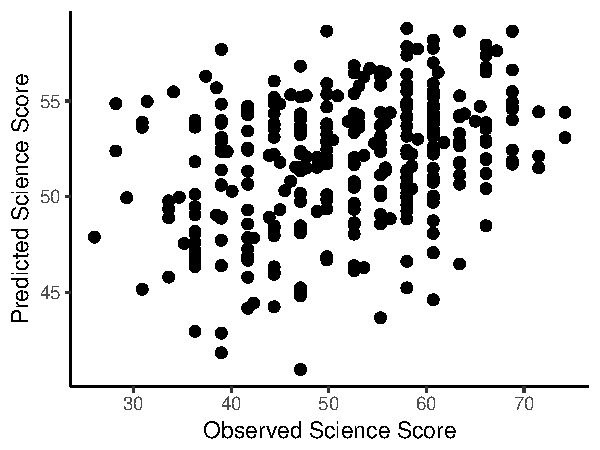
\includegraphics{Homework_3_Revised_Minoo_files/figure-latex/unnamed-chunk-4-1.pdf}

\begin{Shaded}
\begin{Highlighting}[]
\KeywordTok{ggplot}\NormalTok{(hsb1.data, }\KeywordTok{aes}\NormalTok{(concept, }\KeywordTok{residuals}\NormalTok{(hsb1.lm)))+}\StringTok{ }\KeywordTok{geom_point}\NormalTok{(}\DataTypeTok{size =} \DecValTok{2}\NormalTok{) +}\StringTok{ }\KeywordTok{xlab}\NormalTok{(}\StringTok{"Self-Concept"}\NormalTok{) +}\StringTok{ }\KeywordTok{ylab}\NormalTok{(}\StringTok{"Residuals"}\NormalTok{) +}
\StringTok{   }\KeywordTok{theme}\NormalTok{(}
        \DataTypeTok{panel.grid.major =} \KeywordTok{element_blank}\NormalTok{(),}
        \DataTypeTok{panel.grid.minor =} \KeywordTok{element_blank}\NormalTok{(),}
        \DataTypeTok{panel.background =} \KeywordTok{element_blank}\NormalTok{(),}
        \DataTypeTok{panel.border =} \KeywordTok{element_blank}\NormalTok{(),}
        \DataTypeTok{axis.line =} \KeywordTok{element_line}\NormalTok{(),}
        \DataTypeTok{axis.ticks =} \KeywordTok{element_line}\NormalTok{(),}
     \NormalTok{)}
\end{Highlighting}
\end{Shaded}

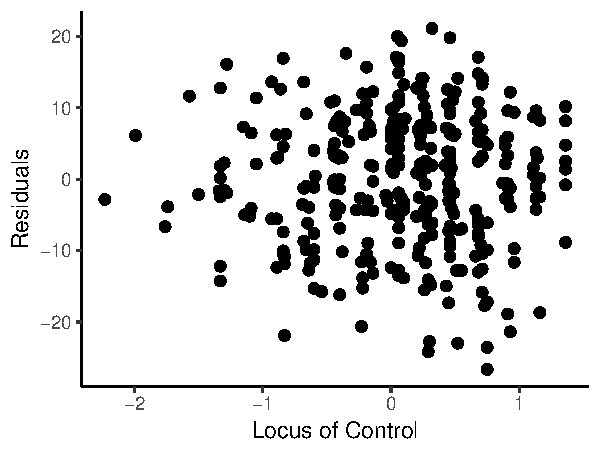
\includegraphics{Homework_3_Revised_Minoo_files/figure-latex/unnamed-chunk-4-2.pdf}

\begin{Shaded}
\begin{Highlighting}[]
\KeywordTok{ggplot}\NormalTok{(hsb1.data, }\KeywordTok{aes}\NormalTok{(mot, }\KeywordTok{residuals}\NormalTok{(hsb1.lm)))+}\StringTok{ }\KeywordTok{geom_point}\NormalTok{(}\DataTypeTok{size =} \DecValTok{2}\NormalTok{) +}\StringTok{ }\KeywordTok{xlab}\NormalTok{(}\StringTok{"Motivation"}\NormalTok{) +}\StringTok{ }\KeywordTok{ylab}\NormalTok{(}\StringTok{"Residuals"}\NormalTok{) +}
\StringTok{   }\KeywordTok{theme}\NormalTok{(}
        \DataTypeTok{panel.grid.major =} \KeywordTok{element_blank}\NormalTok{(),}
        \DataTypeTok{panel.grid.minor =} \KeywordTok{element_blank}\NormalTok{(),}
        \DataTypeTok{panel.background =} \KeywordTok{element_blank}\NormalTok{(),}
        \DataTypeTok{panel.border =} \KeywordTok{element_blank}\NormalTok{(),}
        \DataTypeTok{axis.line =} \KeywordTok{element_line}\NormalTok{(),}
        \DataTypeTok{axis.ticks =} \KeywordTok{element_line}\NormalTok{(),}
     \NormalTok{)}
\end{Highlighting}
\end{Shaded}

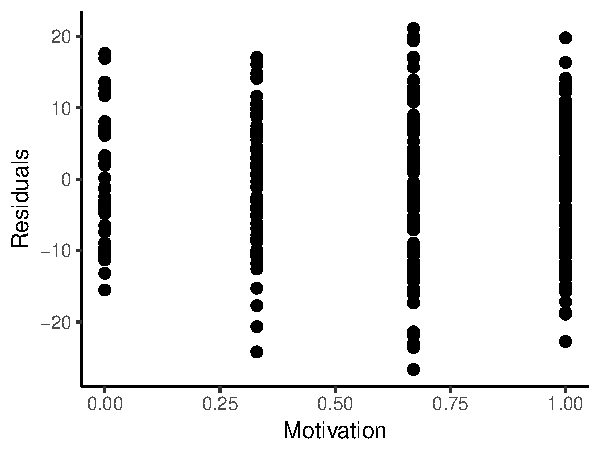
\includegraphics{Homework_3_Revised_Minoo_files/figure-latex/unnamed-chunk-4-3.pdf}

\begin{Shaded}
\begin{Highlighting}[]
\CommentTok{#Plot: Resisulas vs Predicted Y }
\KeywordTok{ggplot}\NormalTok{(hsb1.data, }\KeywordTok{aes}\NormalTok{(}\KeywordTok{fitted.values}\NormalTok{(hsb1.lm), }\KeywordTok{residuals}\NormalTok{(hsb1.lm)))+}\StringTok{ }\KeywordTok{geom_point}\NormalTok{(}\DataTypeTok{size =} \DecValTok{2}\NormalTok{) +}\StringTok{ }\KeywordTok{xlab}\NormalTok{(}\StringTok{"Predicted Y (science score)"}\NormalTok{) +}\StringTok{ }\KeywordTok{ylab}\NormalTok{(}\StringTok{"Residuals"}\NormalTok{) +}\StringTok{ }\KeywordTok{geom_hline}\NormalTok{(}\DataTypeTok{yintercept =} \DecValTok{0}\NormalTok{) +}
\StringTok{   }\KeywordTok{theme}\NormalTok{(}
        \DataTypeTok{panel.grid.major =} \KeywordTok{element_blank}\NormalTok{(),}
        \DataTypeTok{panel.grid.minor =} \KeywordTok{element_blank}\NormalTok{(),}
        \DataTypeTok{panel.background =} \KeywordTok{element_blank}\NormalTok{(),}
        \DataTypeTok{panel.border =} \KeywordTok{element_blank}\NormalTok{(),}
        \DataTypeTok{axis.line =} \KeywordTok{element_line}\NormalTok{(),}
        \DataTypeTok{axis.ticks =} \KeywordTok{element_line}\NormalTok{(),}
     \NormalTok{)}
\end{Highlighting}
\end{Shaded}

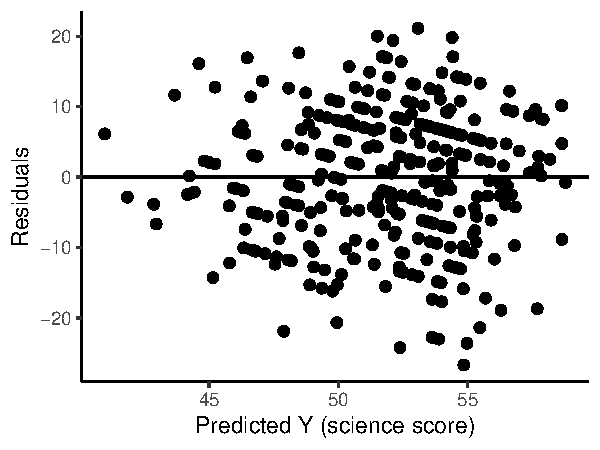
\includegraphics{Homework_3_Revised_Minoo_files/figure-latex/unnamed-chunk-4-4.pdf}

\begin{Shaded}
\begin{Highlighting}[]
\CommentTok{# getting stadardized residuals}
\NormalTok{st.residuals <-}\StringTok{ }\KeywordTok{stdres}\NormalTok{(hsb1.lm)}
\CommentTok{# create residuals hist }
\KeywordTok{hist}\NormalTok{(st.residuals, }\DataTypeTok{freq =} \OtherTok{FALSE}\NormalTok{)}
\KeywordTok{curve}\NormalTok{(dnorm, }\DataTypeTok{add =} \OtherTok{TRUE}\NormalTok{)}
\end{Highlighting}
\end{Shaded}

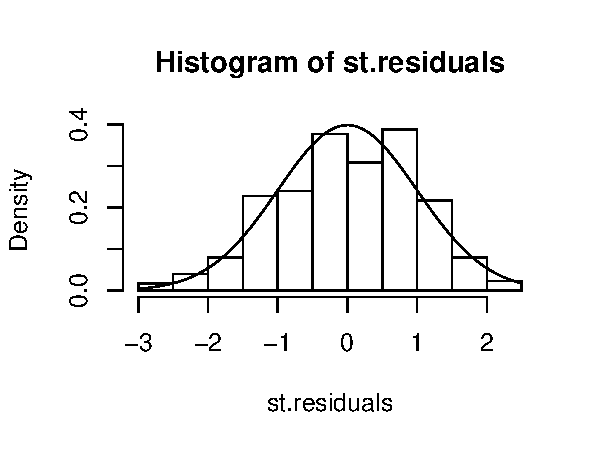
\includegraphics{Homework_3_Revised_Minoo_files/figure-latex/unnamed-chunk-4-5.pdf}

\begin{Shaded}
\begin{Highlighting}[]
\CommentTok{# create PP plot}
\KeywordTok{ggplot}\NormalTok{(hsb1.data, }\KeywordTok{aes}\NormalTok{(}\DataTypeTok{sample =} \NormalTok{st.residuals))+}\StringTok{ }\KeywordTok{stat_qq}\NormalTok{() +}\StringTok{ }\KeywordTok{geom_abline}\NormalTok{(}\DataTypeTok{intercept =} \DecValTok{0}\NormalTok{, }\DataTypeTok{slope =} \DecValTok{1}\NormalTok{) +}
\StringTok{   }\KeywordTok{theme}\NormalTok{(}
        \DataTypeTok{panel.grid.major =} \KeywordTok{element_blank}\NormalTok{(),}
        \DataTypeTok{panel.grid.minor =} \KeywordTok{element_blank}\NormalTok{(),}
        \DataTypeTok{panel.background =} \KeywordTok{element_blank}\NormalTok{(),}
        \DataTypeTok{panel.border =} \KeywordTok{element_blank}\NormalTok{(),}
        \DataTypeTok{axis.line =} \KeywordTok{element_line}\NormalTok{(),}
        \DataTypeTok{axis.ticks =} \KeywordTok{element_line}\NormalTok{(),}
     \NormalTok{)}
\end{Highlighting}
\end{Shaded}

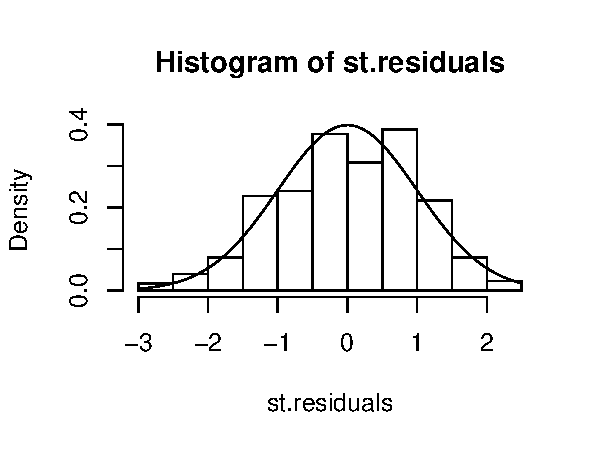
\includegraphics{Homework_3_Revised_Minoo_files/figure-latex/unnamed-chunk-4-6.pdf}

\begin{Shaded}
\begin{Highlighting}[]
\CommentTok{# qq plot for studentized residuals}
\KeywordTok{qqPlot}\NormalTok{(hsb1.lm, }\DataTypeTok{main =} \StringTok{"QQ plot"}\NormalTok{)}
\end{Highlighting}
\end{Shaded}

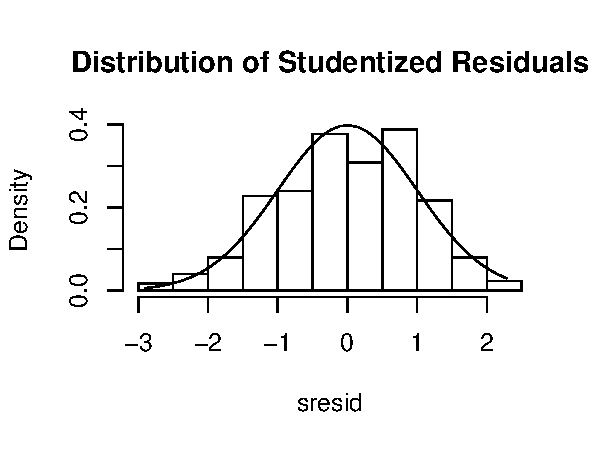
\includegraphics{Homework_3_Revised_Minoo_files/figure-latex/unnamed-chunk-4-7.pdf}

\begin{center}
\Large \textbf{Part 2: Multiple Regression - Final model: Use data set HSB1}
\end{center}

\begin{enumerate}
\def\labelenumi{\arabic{enumi}.}
\item
  I tried BoxCox and BoxTidwell to achieve linearity, also tried taking
  logs to correct for the skewness, but neither of these changed the
  t-value for the two non-significant predictors (concept and
  motivation) significantly and they still remained non-significant. For
  the other types of regression (WLS) I couldn't find helpful resources
  on the internet, mainly because they were too advanced for me.
\item
  This research was designed to determine the influence of locus of
  control, self-concept and motivation on science score. Students'
  science scores were regressed on their scores for locus of control,
  self-concept and motivation. The overall multiple regression was
  statistically significant
  (\(R^2 = 0.1139, F(3, 346) = 14.83, p < 0.001\)). The three variables
  (locus of control, self-concept and motivation) accounted for 11\% of
  the variance in science score. From among these three variable, only
  locus of attention had a statistically significant effect on the
  science score. The unstandardized regression coefficient ( \(\beta\))
  for locus of control was 4.7188 ( \(t(346)= 6.068, p < 0.001\) ),
  meaning that for each additional score on locus of control, students'
  science score increased by 4.7188 points, controlling for on
  self-concept and motivation. These results suggest that locus of
  control is indeed an important influence on students' science grade
  and that this effect holds even after students' self-concept and
  motivation are taken into account. Students who want to improve their
  grades in science may do so by increasing their locus of contorl.
\end{enumerate}

\begin{table}[H]
\centering
\begin{tabular}{c|c|c}
Variable & B & SE B \\\hline
Locus & 4.7188\text{**} & 0.7776\\
Concept & 0.2549 & 0.7606\\
Motivation & 1.7113 & 1.4978
\end{tabular}
\caption{\label{tab:widgets}Summary of Regression Analysis for Variables Predicting Science Score. ** p-value< 0.01}
\end{table}

\begin{center}
\Large \textbf{Part 3: ANOVA using Multiple Regression}
\end{center}

\begin{enumerate}
\def\labelenumi{\arabic{enumi}.}
\tightlist
\item
  \[\hat{Y} = 97.8 + 7.7(\text{Tretment A}) + 2.7(\text{Tretment B}) + 5.7(\text{Tretment C})\]
\end{enumerate}

The intercept shows the mean score for Treatment D (our reference). Each
of the other coefficients in the model represents the difference between
mean score for that treatment with the mean score for Treatment D.

\begin{enumerate}
\def\labelenumi{\arabic{enumi}.}
\setcounter{enumi}{1}
\item
\end{enumerate}

\(H_0\):
\(\mu_\text{treatment A} = \mu_\text{treatment B} =\mu_\text{treatment C} =\mu_\text{treatment D}\)

\(H_1\): At least one of group means is different from
\(\mu_\text{treatment D}\).

We failed to reject the null, since none of the mean scores in either of
the treatment groups was significantly different from the mean score in
Treatment D. (all t-values\textless{}1.4 and all
p-values\textgreater{}.05).

\begin{enumerate}
\def\labelenumi{\arabic{enumi}.}
\setcounter{enumi}{2}
\tightlist
\item
  \[\hat{Y_D} = 97.8 + 7.7(0) + 2.7(0) + 5.7(0) = 97.8\] The mean score
  in Treatment D is 97.8.
\end{enumerate}

\[\hat{Y_B} = 97.8 + 7.7(0) + 2.7(1) + 5.7(0) = 100.5\] The mean score
for Treatment B is 100.5.


\end{document}
